\documentclass[11pt]{article}
\usepackage[english]{babel}  % Croatian typographical rules and hyphenation patterns
\usepackage{ae,aecompl}     	% Type 1 fonts, similar to Computer Modern

\usepackage{microtype}				% Improves spacing

\usepackage{booktabs}					% Nice looking tables
\usepackage{enumerate}				% Additional options for listing of items in enumerate environment
\usepackage{algorithm2e}			% Writing pseudo-code
\usepackage{todonotes}				% Adding todo items
\usepackage{dirtree}					% Simple display of directory tree
\usepackage{hyperref}

\usepackage{graphicx}
\usepackage{subfig}
\usepackage{caption}
\usepackage{listings}

\hypersetup{
    colorlinks=true,
    linkcolor=blue,
    filecolor=magenta,
    urlcolor=cyan,
}
\urlstyle{same}
\usepackage{graphics}

\graphicspath{ {./images/} }

\title{
	\Large Josip Juraj Strossmayer University of Osijek \\
	Faculty of Electrical Engineering, Computer Science and Information
	 Technologies\\
	\vspace{4cm}
	\Large Course: Linux in Embedded Systems \\
	\vspace{4cm}
	\Large \textbf{Laboratory exercise 3: Nunchuk - I\textsuperscript{2}C device}
	}
\date{}
\begin{document}
\maketitle
\thispagestyle{empty}
\newpage

\section{Introduction}
The goal of this exercise is to identify the I\textsuperscript{2}C device in
the Linux operating system and create a basic kernel module that will be
upgraded in the next laboratory exercises. The goal is also to create a device
tree. Also, it is necessary to create a kernel module with basic versions of
\texttt{probe()} and \texttt{remove()} functions.

\section{Connecting Nunchuk to Raspberry Pi}
Get the Nunchuk device you received from the assistant.
Using the connectors, we will connect the Nunchuk device to the Raspberry Pi J8
pins
You can download documents with useful information about Nunchuk from
addresses:\\
\url{https://bootlin.com/labs/doc/nunchuk.pdf}\\
\url{https://www.robotshop.com/media/files/PDF/inex-zx-nunchuck-datasheet.pdf}\\

\begin{figure}[h!]
\centering
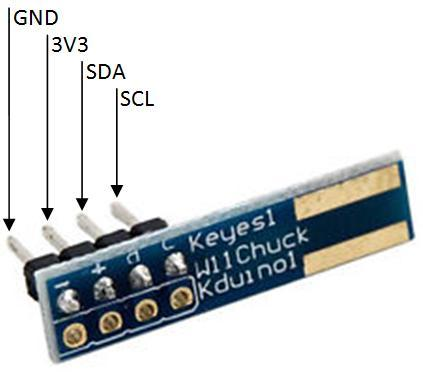
\includegraphics[width=0.4\textwidth]{nunchuk-connector.jpg}
\captionsetup{justification=centering}
\caption{Nunchuk connector pin layout}
\end{figure}

\begin{figure}[h!]
\centering
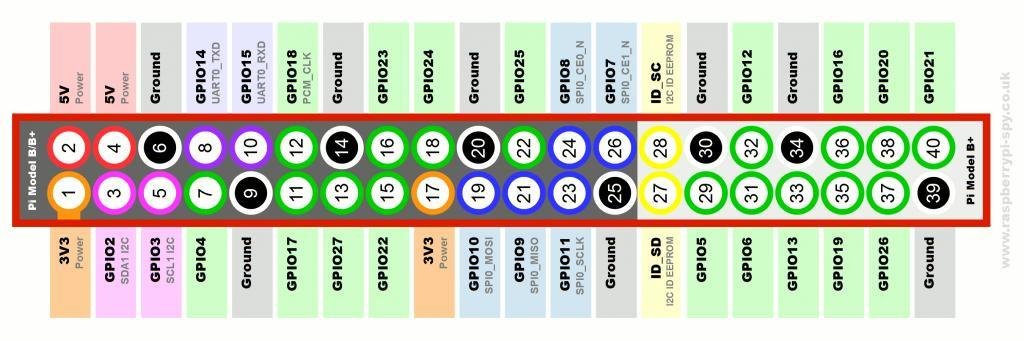
\includegraphics[width=0.95\textwidth]{j8-rpi.jpg}
\captionsetup{justification=centering}
\caption{Pin layout of J8 connectors on Raspberry Pi 3 board}
\end{figure}

Now connect the Nunchuk connector and the Raspberry Pi 3 board as follows:
\begin{itemize}
	\item GND pin to J8 pin 9 (GND),
	\item 3V3 pin to J8 pin 1 (3V3),
	\item SCL pin to J8 pin 5 (GPIO3/SCL1 I2C),
	\item SDA pin to J8 pin 3 (GPIO2/SDA1 I2C).
\end{itemize}

\section{Creating a custom device tree}
To allow Linux kernel to handle a new device, we need to add a description of
that device in the board device tree. As the device tree for the Raspberry Pi 3
board is already included in the Linux kernel, we will not make changes directly
to the file already used for this board, but will create a special device tree
for our board with our device.

Go to the directory where Linux source code is, that should be in the path\\
\texttt{/home/profesor/buildroot/output/build/linux-custom}. Make a copy of\\
\texttt{bcm2710-rpi-3-b.dts} file located in the \texttt{arch/arm/boot/dts} and
name it \texttt{bcm2710-rpi-3-b-custom.dts}. Make changes to the
\texttt{Makefile} in the same directory and allow the new dts file to be
compiled as well.
\newline
\newline
Within the new device tree file, we first need to enable the \texttt{i2c1} bus.
Next, declare the \texttt{nunchuk} device as the \texttt{i2ci} successor node.
Use \texttt{nintendo,nunchuk} for the compatible property. I\textsuperscript{2}C
register address of the Nunchuk device can be found in the Nunchuk document.
\newline
\newline
After the necessary modifications, the \texttt{i2c1} node should look like this:
\begin{lstlisting}[language=bash]
&i2c1 {
	pinctrl-names = "default";
	pinctrl-0 = <&i2c1_pins>;
	clock-frequency = <100000>;
	status="okay";

	nunchuk: nunchuk@52 {
		compatible ="nintendo,nunchuk";
		reg = <0x52>;
		status = "okay";
	};
};
\end{lstlisting}
After making the necessary changes to the device tree file, position yourself
in the root path of the Linux source code:\\
(\texttt{/home/profesor/buildroot/output/build/linux-custom}).\\
Set the environment variables required to compile the Linux kernel:
\begin{lstlisting}
export ARCH=arm
export CROSS_COMPILE=arm-linux-gnueabihf-
\end{lstlisting}
After that, start compiling the device tree files using the command:
\begin{lstlisting}
make dtbs
\end{lstlisting}
Copy the new dtb file to the \texttt{tftp} server directory\\
(\texttt{/var/lib/tftpboot}) and make the necessary changes to the Uboot
configuration for the Raspberry Pi board to load a new device tree during boot.
\newline
\newline
Through the \texttt{/proc/device-tree} directory, we can check all the device
tree settings that our system has loaded.
\newline
For example, we can check the presence of a \texttt{nunchuk} node in the device
tree:
\begin{lstlisting}
# find /proc/device-tree/ -name "*nunchuk*"
/proc/device-tree/soc/i2c@7e804000/nunchuk@52
\end{lstlisting}
Some settings of the device could be read like this:
\begin{lstlisting}
cat /proc/device-tree/soc/i2c@7e804000/nunchuk@52/status
\end{lstlisting}

\section{Writing simple device driver}
You can now start creating a driver for \textit{Nunchuk}. In the
\texttt{/home/profesor/embedded\_linux/LV3/solutions} directory, create a
\texttt{nunchuk} directory. Create two files inside that directory:
 \texttt{nunchuk.c} and \texttt{Makefile}.
\newline
\newline
Makefile file structure is standard. An essential parameter is KDIR, which
 indicates the path to the Linux kernel source.
\newline
\newline
The following should be implemented within the \texttt{nunchuk.c} file:
\begin{enumerate}
	\item \texttt{probe()} and \texttt{remove()} functions to be called when
		\texttt{nunchuk} is found or removed. For now, just use the
		\texttt{printk()} call within functions to confirm that the functions
		have been called.
	\item Initialize \texttt{i2c\_device\_id} structure. After that, call the
		\texttt{MODULE\_DEVICE\_TABLE} macro function. Check what that helper
		macro function does.
	\item Initialize \texttt{i2c\_driver} structure and register
		I\textsuperscript{2}C driver using same. compatible settings must match
		those from the device tree. Invoke \texttt{module\_i2c\_driver} macro
		function with previously initialized \texttt{i2c\_driver} structure.
		Check what that helper macro function does.
\end{enumerate}
Compile the kernel module (\texttt{ARCH} and \texttt{CROSS\_COMPILE} environment
 variables must be set previously) using the command:
\begin{lstlisting}
make
\end{lstlisting}
Copy the created nunchuk.ko kernel module to the NFS path\\
\texttt{/home/profesor/embedded\_linux/LV2/solutions/nfsroot/root}. Insert and
 remove kernel module using the \texttt{insmod} and \texttt{rmmod} commands.

\section{Saving work}
Position yourself in the \texttt{/home/profesor/embedded\_linux/LV3/solutions/nunchuk}
 directory.
Execute \texttt{Git} Commands:
\begin{lstlisting}
git add nunchuk.c
git add Makefile
git commit -m "laboratory exercise 3 done"
git push origin master
\end{lstlisting}
\end{document}
